\section{Information theory quantifiers}\label{sec:quanti}

All the statistical quantifiers studied here are functionals of the PDF associated to the time series.
The first step to quantify the statistical properties of the values (amplitude statistics) of a time series $\{x_i,~(i=1,...,N)\}$ using information theory is to determine the concomitant PDF.
This is an issue studied in detail in previous papers \cite{aka varios}.
Let us summarize the procedure:

\begin{enumerate} 
\item \label{1} a finite alphabet with $M$ symbols $\mathcal{A}=\{a_1,...,a_M\}$ is chosen. 
\item \label{2} one of these symbols is assigned to each: (a) value of the time series or (b)portion of length $D$ of the trajectory. 
\item \label{3} the normalized histogram of the symbols is the desired PDF.
\item \label{4} an ramdomness quantifier is calculated over desired PDF. In our case we calculate (a) normalyzed Shannon entropy $H$, (b) normalyzed statistical complexity $C$ and (d) missing patterns $MP$.
\end{enumerate}

Note that if option (a) is chosen in step \ref{2} then the PDF is \textit{non causal}, because all the information about the time evolution of the system generating $\{x_i\}$ is completely lost.
On the contrary if option (b) is chosen in step \ref{2} then the PDF is \textit{causal}, in the sense it includes information about the temporal evolution.

\textcolor{red}{NOMBRAR DE LA BPW, SI ES QUE LA TERMINAMOS USANDO}

\textcolor{red}{NOMBRAR LOS PLANOS QUE TERMINEMOS ELIGIENDO}

Of course there are infinite possibilities to choose the alphabet $\mathcal{A}$ as well as the length $D$.
Bandt \& Pompe made a proposal for a causal PDF that has been shown to be easy to implement and useful in a great variety of applications \textcolor{red}{REFERENCIAS A APLICACIONES}.
The procedure is the following \cite{Bandt2002,Keller2003,Keller2005}: \textcolor{red}{ESTA PARTE ESTÁ EN EL TIEMPO Y DEBERÍA ESTAR EN LAS MUESTRAS}

\begin{itemize}
\item Given a series $\{x_t : t=0, \Delta t, \cdots,M\Delta t \}$, a sequence of vectors of length $D$ is generated.

\begin{equation}
\label{eq:vectores}
(s)\mapsto \left(x_{t-(d-1)\Delta t},x_{t-(d-2)\Delta t},\cdots,x_{t-\Delta t},x_{t}\right) \ ,
\end{equation}

Each vector turns out to be the ``history'' of the value $x_t$. Clearly, the longer the length of the vectors $D$, the more information about the history would the vectors have but a higher value of $N$ is required to have an adequate statistics. 

\item The permutations $\pi=(r_0, r_1, \cdots, r_{D-1})$ of $(0, 1, \cdots, D-1)$ are called ``order of patterns'' of time $t$, defined by:

\begin{equation}
\label{eq:permuta}
x_{t-r_{D-1}\Delta t}\le x_{t-r_{D-2}\Delta t}\le\cdots\le x_{t-r_{1}\Delta t}\le x_{t-r_0\Delta t}.
\end{equation}

In order to obtain an unique result it is considered $r_i<r_{i-1}$ if $x_{t-r_{i}\Delta t}=x_{t-r_{i-1}\Delta t}$.

In this way, all the $D!$ possible permutations $\pi$ of order $D$, and the PDF $P=\{p(\pi)\}$ is defined as:

\begin{equation}
\label{eq:frequ}
p(\pi)=\frac{\sharp \{s|s\leq M-D+1; (s) \quad \texttt{has type}~\pi\}}{M-D+1}.
\end{equation}

In the last expression the $\sharp$ symbol means ``number".
\end{itemize}

This procedure has the advantages of being {\it i)} simple, {\it ii)} fast to calculate, {\it iii)} robust in presence of noise, and {\it iv)} invariant to lineal monotonous transformations. \textcolor{red}{DICE QUE ES ROBUSTO FRENTE A LA PRESENCIA DE RUIDO PERO NO, REFERENCIAS?}

It is applicable to weak stationarity processes (for $k=D$, the probability that $x_t < x_{t+k}$ doesn't depend on the particulary $t$ \cite{Bandt2002}).The causality property of the PDF allows the quantifiers (based on this PDFs) to discriminate between deterministic and stochastic systems \cite{Rosso2007B}.

According to this point Bandt and Pompe suggested $3\leq D \leq 7$. $D=6$ has been adopted in this work.

\textcolor{red}{HABLAR DE BPW}

The entropy $H[P]$ is the normalized version of the Entropy proposed by Shannon \cite{Shannon1948}:
\begin{equation}\label{eq:sha}
H[P] = S[P] /S_{max},
\end{equation}
where $S[P]=-\sum _{j=1}^{M}~p_j~\ln( p_j )$\\ and $S_{max}$ is
the normalizing constant:
\begin{equation}
\label{eq:Smax} S_{max}= S[P_e] = \ln M,
\end{equation}
and $P_e=\{ 1/M, \cdots,1/M\}$ is the uniform distribution.

The statistical complexity $C[P]$ is given by:
\begin{equation}
\label{eq:inten}
C[{P}]=Q_{J}[{P,P_e}]\cdot H[{P}] \ ,
\end{equation}
, and
$Q_{J}$ is named ``disequilibrium'' and it is the distance between $P$ and $P_e$ in the probability space.
The metric used in this paper is based on the Jensen-Shannon divergence \cite{Lamberti2004}:
\begin{equation}
\label{eq:disequi}
Q_{J}[{P,P_e}]= Q_0 \cdot \{S[\frac{P+P_e}{2}]-S[P]/2-S[P_e]/2 \} \ .
\end{equation}
The normalization constant $Q_0$ is:
\begin{equation}
\label{eq:q0j}
Q_0=-2 \left\{ \left( \frac{N+1}{N} \right) \ln(N+1) - 2 \ln(2N) + \ln N \right\}^{-1} .
\end{equation}

From the statistical point of view the disequilibrium $Q_J$ is an intensive magnitude, and it is $0$ if and only if $P=P_e$.
It has been proved that the $C[P]$ quantifies the presence of nonlinear correlations typical of chaotic systems \cite{Martin2003,Lamberti2004}.
The complexity $C[P]$ is independent from the entropy $H[P]$, as far as different $P$'s share the same entropy $H[P]$ but they have different complexity $C[P]$.

\textcolor{red}{PONER UN PÁRRAFO QUE ENGANCHE LAS H's Y C's CON LOS HISTOGRAMAS PARA ARMAR Hval, Cval, Hbp, Cbp, Hbpw y Cbpw}

The number of symbols $M$ is equal to $N$ for $H_{hist}$ and it is equal to $D!$ for $H_{BP}$ and $H_{BPW}$.

Two representation planes are considered: $H_{BP}$ vs $H_{hist}$ \cite{DeMicco2008} and $H_{BP}$ vs $C_{BP}$ \cite{Rosso2007}.
In the first plane a higher value in any of the entropies, $H_{BP}$ and $H_{hist}$, implies an increase in the uniformity of the involved PDF.
The point $(1,1)$ represents the ideal case with uniform histogram and uniform distribution of ordering patterns.
In the second plane not the entire region $0<H_{BP}<1$, $0<C_{BP}<1$ is achievable.
In fact for any PDF the pairs $(H,C)$ of possible values fall between two extreme curves in the plane $H$-$C$ \cite{Anteneodo1996}.
Fig. \ref{fig:CbpHbp} shows two regions labeled as \textit{deterministic} and \textit{stochastic}.
In fact transition from one region to the other are smooth and the division is a bit arbitrary.
A more detailed discussion can be seen in \cite{Rosso2007}.
Ideal random systems having uniform Bandt \& Pompe PDF, are represented by the point $(1,0)$ \cite{Gonzalez2005} and a delta-like PDF corresponds with the point $(0,0)$.

\begin{figure}
	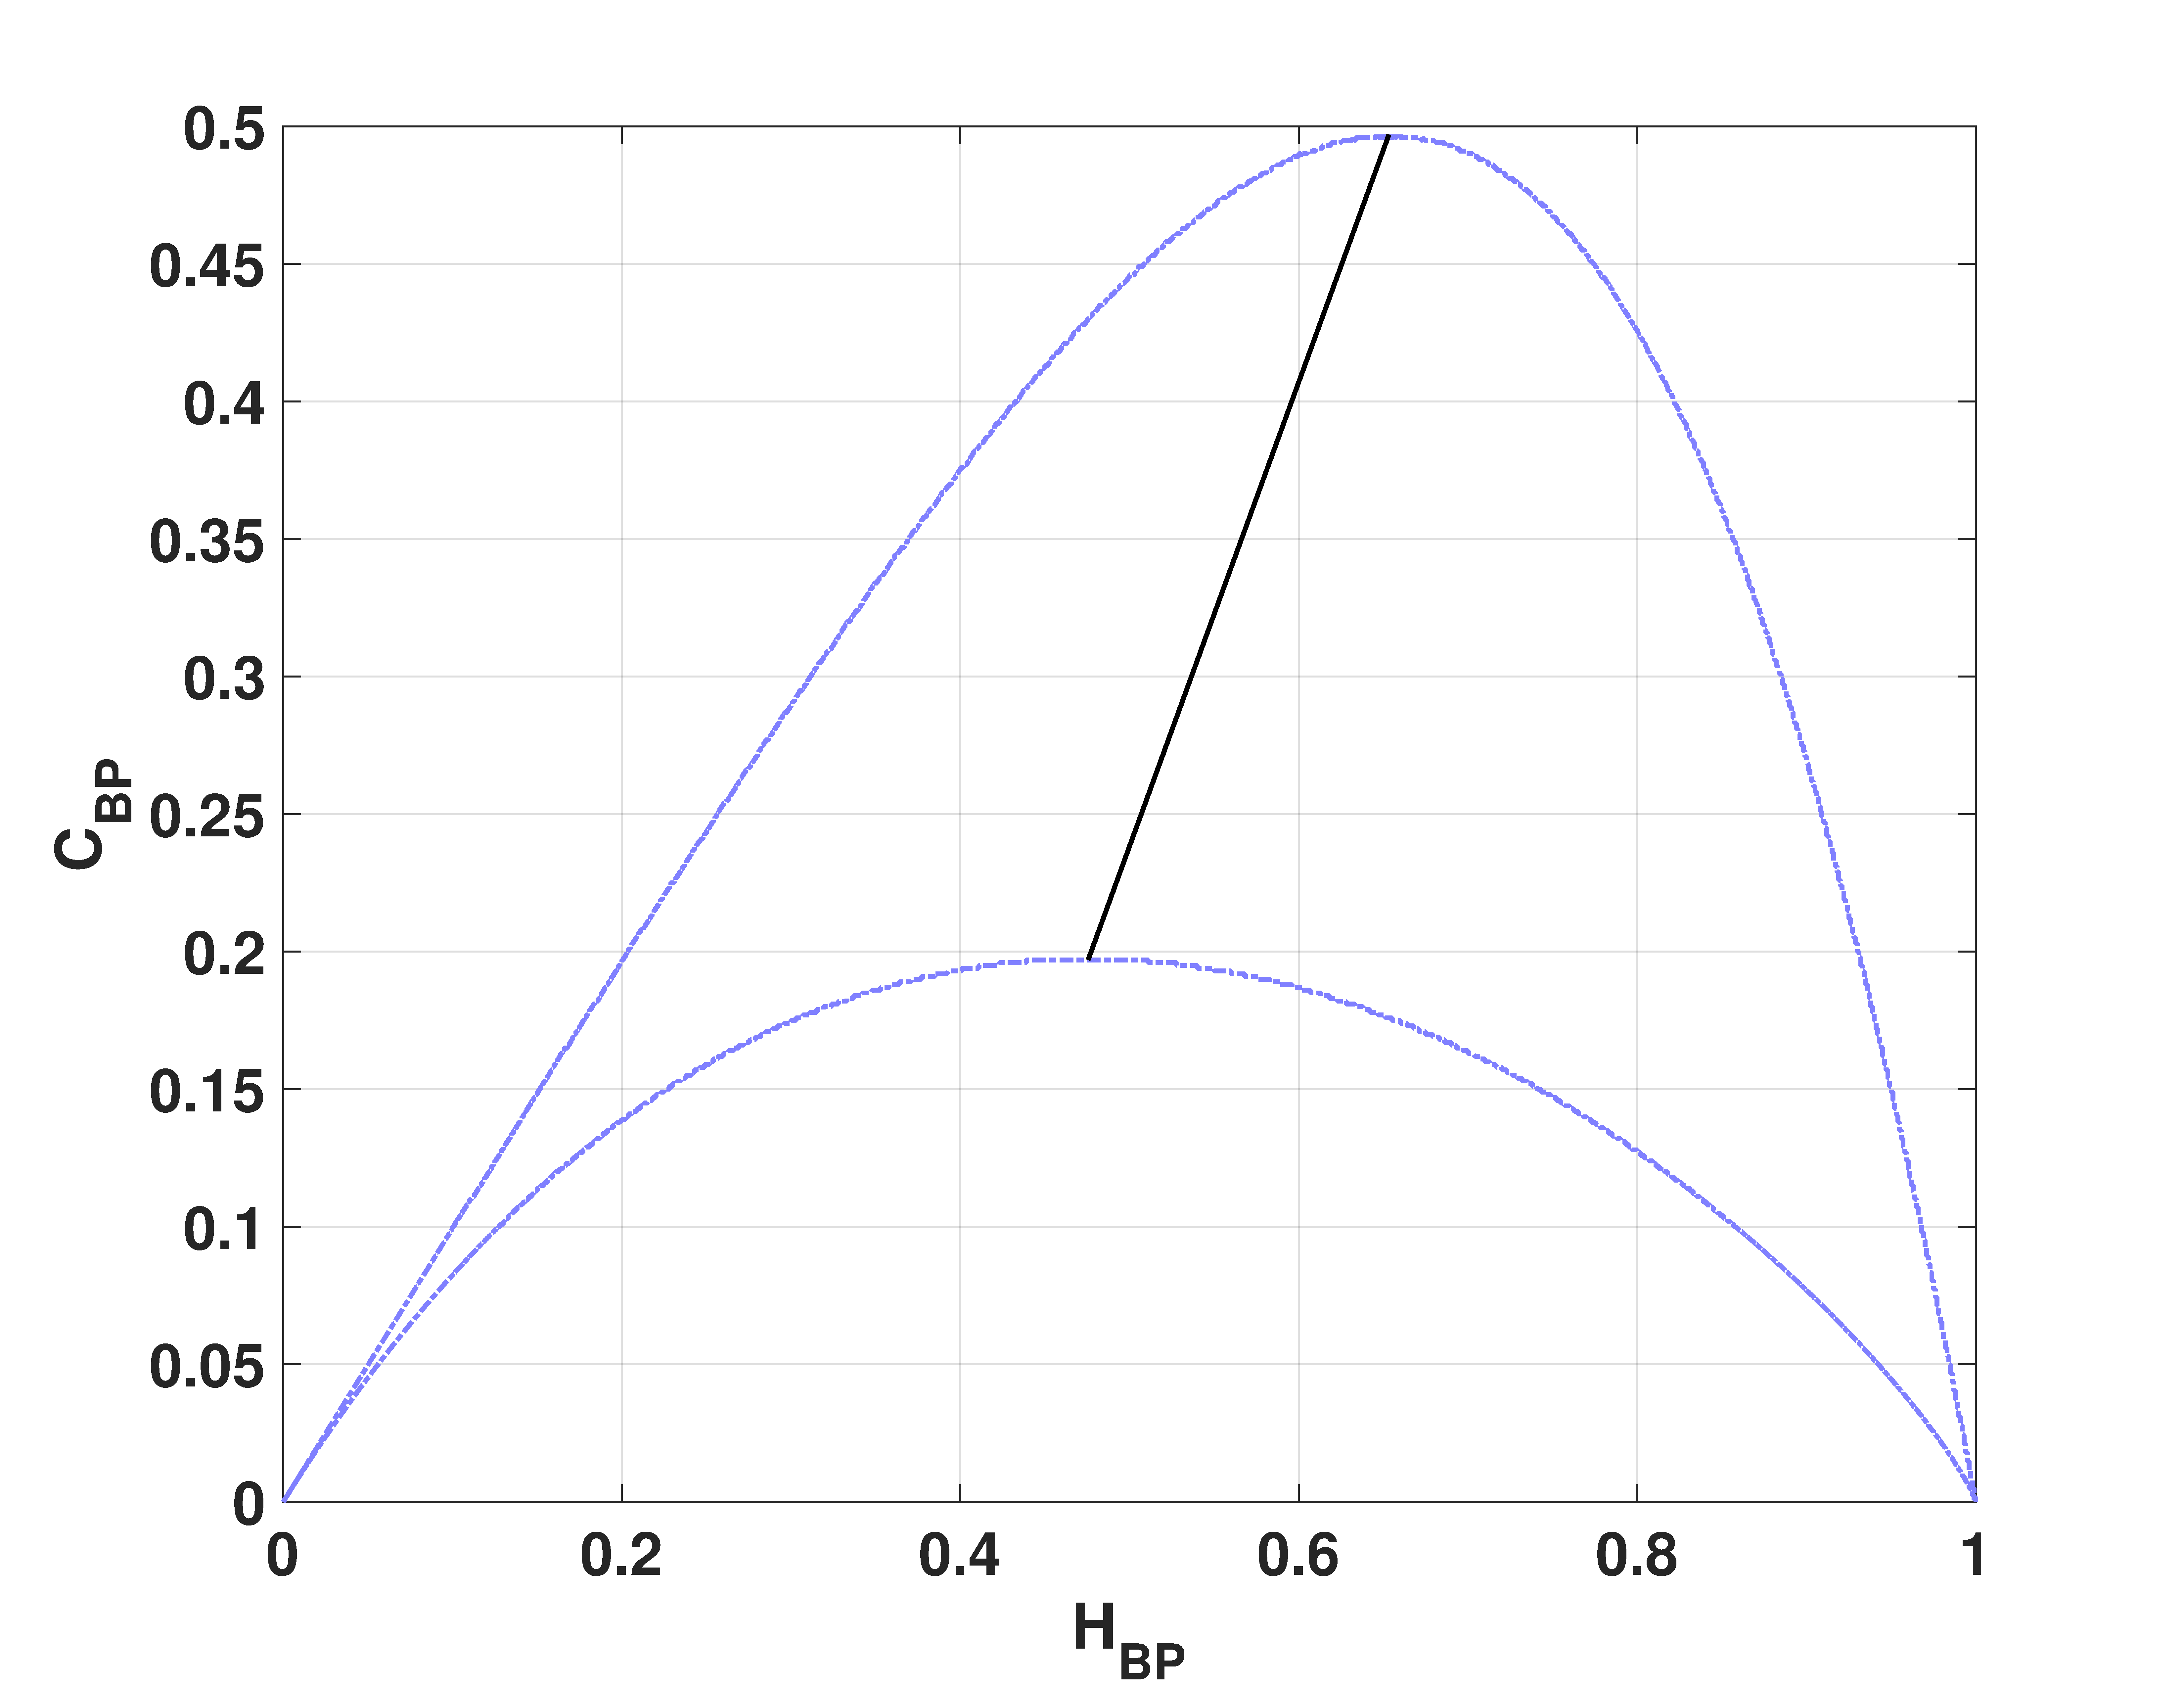
\includegraphics[width= .49\textwidth]{CbpHbp}
	\caption{Entropy-Complexity plane.}
	\label{fig:CbpHbp}
\end{figure}

We also used the number of missing patterns $MP$ as a quantifier\cite{Rosso2012}.
As shown recently by Amig\'o {\it et al.} \cite{Amigo2006,Amigo2007,Amigo2008,Amigo2010}, in the case of deterministic one-dimensional maps, not all the possible ordinal patterns can be effectively materialized into orbits, which in a sense makes these patterns ``forbidden".
Indeed, the existence of these {\it forbidden ordinal patterns} becomes a persistent fact that can be regarded as a ``new" dynamical property.
Thus, for a fixed pattern-length (embedding dimension $D$) the number of forbidden patterns of a time series (unobserved patterns) is independent of the series length $N$.
Remark that this independence does not characterize other properties of the series such as proximity and correlation, which die out with time \cite{Amigo2007,Amigo2010}.

A full discussion about the convenience of using these quantifiers is out of the scope of this work.
Nevertheless reliable bibliographic sources do exist \cite{Wackerbauer1994,Lopez-Ruiz1995,Rosso2007A,DeMicco2008,Rosso2010,Martin2006,Rosso2012}.